\documentclass[tikz,convert={outfile=\jobname.svg}]{standalone}
\usetikzlibrary{patterns}
\begin{document}
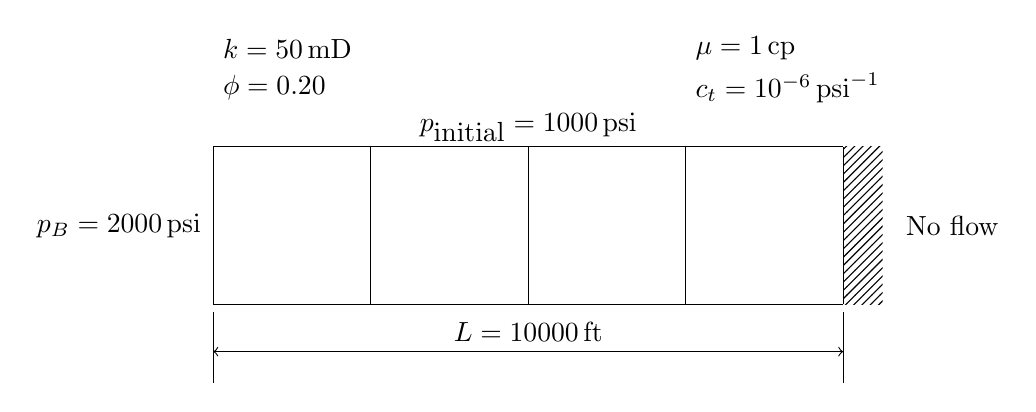
\begin{tikzpicture}
\foreach \i in {0, 2, 4, 6, 8} {%
    \draw [] (\i,0) -- (\i,2)  node [below] at (\i,0) {};
}
\foreach \i in {0, 8} {%
    \draw (\i, -0.1) -- (\i, -1);
}
\foreach \i in {0, 2} {
    \draw [] (0,\i) -- (8,\i) node [left] at (0,\i) {};
}
\draw [right] node at (0,3.25) {$k = 50\,$mD};
\draw [right] node at (0,2.75) {$\phi=0.20$};
\draw [right] node at (6,3.25) {$\mu = 1\,$cp};
\draw [right] node at (6,2.75) {$c_t=10^{-6}\,\mbox{psi}^{-1}$};
\draw [] node at (4,2.25) {$p_{\mbox{initial}} = 1000\,$psi};
\draw [] node at (-1.2,1) {$p_{B} = 2000\,$psi};
\draw[<->] (0,-0.6) -- (8,-0.6) node[draw=none,fill=none, midway, above] {$L=10000\,$ft};
\fill [pattern=north east lines] (8,0) rectangle (8.5,2) node [label={[label distance=0.3cm]0:No flow}, midway] {};
\end{tikzpicture}
\end{document}
